\section{k-Nearest Neighbors and Cross-validation \problemworth{20}}
In the following questions you will consider a $k$-nearest neighbor classifier using the Euclidean distance metric on a binary classification task. We assign the class of the test data point to be the class of the majority of the $k$ nearest neighbors. Note that when the test data point is the same as one of the training data point. That training data point can be consider as the closet neighbor of the test data point. 

\begin{figure}[h]
    \centering
    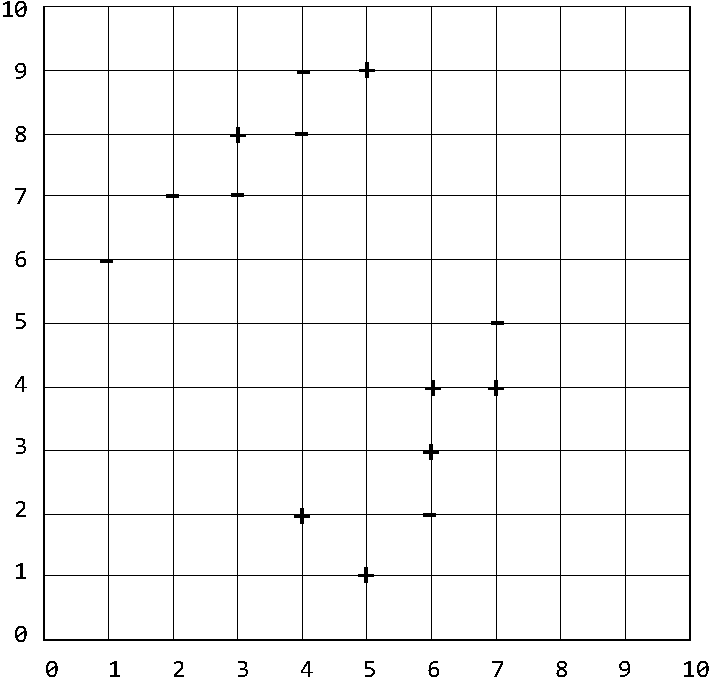
\includegraphics[scale=0.8]{knn_figure.pdf}
    \caption{Dataset for KNN binary classification task.}
    \label{fig:knn}
\end{figure}

\begin{enumerate}
 \item \itemworth{5} 
        What will be the label of point (5,9) in Fig \ref{fig:knn} using k-NN algorithm with majority voting when $k=1$?


    \item \itemworth{5} 
        What will be the label of point (5,9) in Fig \ref{fig:knn} using k-NN algorithm with majority voting when $k=3$?

    \item \itemworth{10}
        Draw the decision boundary of k-NN when $k=1$ on Fig \ref{fig:knn}.

\end{enumerate}